\chapter*{Заключение}						% Заголовок
\addcontentsline{toc}{chapter}{Заключение}	% Добавляем его в оглавление

%% Согласно ГОСТ Р 7.0.11-2011:
%% 5.3.3 В заключении диссертации излагают итоги выполненного исследования, рекомендации, перспективы дальнейшей разработки темы.
%% 9.2.3 В заключении автореферата диссертации излагают итоги данного исследования, рекомендации и перспективы дальнейшей разработки темы.
%% Поэтому имеет смысл сделать эту часть общей и загрузить из одного файла в автореферат и в диссертацию:

Основные результаты работы заключаются в следующем.
%% Согласно ГОСТ Р 7.0.11-2011:
%% 5.3.3 В заключении диссертации излагают итоги выполненного исследования, рекомендации, перспективы дальнейшей разработки темы.
%% 9.2.3 В заключении автореферата диссертации излагают итоги данного исследования, рекомендации и перспективы дальнейшей разработки темы.

В процессе разработки аппаратуры для радиационного мониторинга на борту космического аппарата были выделены основные требования к дозиметру, которые позволили создать прибор ДЭПРОН, удовлетворяющий и выполнению задачи мониторинга обстановки и исследовательским целям в космической дозиметрии. Для решения этой задачи был проведен анализ современной литературы по направлению космической дозиметрии. Были найдены аналоги создаваемого прибора и определен ряд критических параметров для такого типа приборов, в том числе энергетические диапазоны регистрируемых излучений, типы излучений и ориентировочные потоки в изучаемых областях космического пространства. Эти параметры и определили оптимальные размеры детекторов, их расположение и требуемое быстродействие встраиваемых вычислительных процессоров.

Для выполнения поставленных задач был создан активный дозиметр нового типа с возможностью регистрации нейтронов тепловых энергий.

Средняя доза на 

\section{Выводы}
\begin{enumerate}
	\item Систематизированы и обобщены характеристики радиационных условий на аналогичных орбитах (аппараты БИОН, Прогноз, Cluster, POES) для разработки программы эксперимента;
	\item Разработаны требования к бортовому дозиметру для нового пилотируемого транспортного корабля;
	\item Разработан прибор для дозиметрического мониторинга на борту космического аппарата <<Ломоносов>>;
	\item Подготовлен и проведен эксперимент с дозиметром на борту КА <<Ломоносов>>;
	\item Обработана полученная с прибора ДЭПРОН информация и проведен её анализ.	
\end{enumerate}

Дополнительные результаты, полученные в результате проведения эксперимента ДЭПРОН: 
\begin{enumerate}

  \item Приближенные оценки показали, что полупроводниковые детекторы прибора чувствительны к электронам энергий более 0,5 МэВ и протонам с энергиями более 5 МэВ;
  \item Математическое моделирование показало что максимум функции чувствительности нейтронный счетчиков соответствует энергии нейтронов 0,005 МэВ и 0,05 МэВ детекторов различной защищенности;
  \item Поглощенная доза за время проведения эксперимента достигла ... и ... для верхнего и нижнего детекторов.
  
\end{enumerate}

\section{Благодарности}
Автор выражает благодарность научному руководителю Бенгину В.В. прошедшему огромный путь вместе с диссертантом, и поддерживавшим словом и делом каждый момент времени. 

Также Золотарев И.А. выражает благодарность Панасюку М.И., давшему возможность включиться в большой образовательный проект - создание спутника Ломоносов и разрабатывать аппаратуру радиационного мониторинга. Также автор благодарен обучению которое обеспечили  все участники коллаборации космического эксперимента: Яшин И.В., Петров В.Л., Амелюшкин А.М. и другие.  Автор благодарен коллегам  лаборатории Нечаеву О.Ю. и Братолюбовой Л.С. за руководство и поддержку. Особую благодарность автор выражает Нечаеву О.Ю. и Смирнову Л.А. за то что они,  своими руками, создали надежный прибор, который лег в основу настоящей диссертационной работы.

Автор благодарен за всемерную поддержку при подготовке диссертации Логачева Ю.И., Южкова Б.Ю. и Оседло В.И. и всех сотрудников отдела ОКФИ НИИЯФ МГУ.  

В заключение хочется отметить что данная работа была бы невозможна без всемерной поддержки жены автора Золотаревой Любови Святославовны.

\begin{figure}
	\centering
	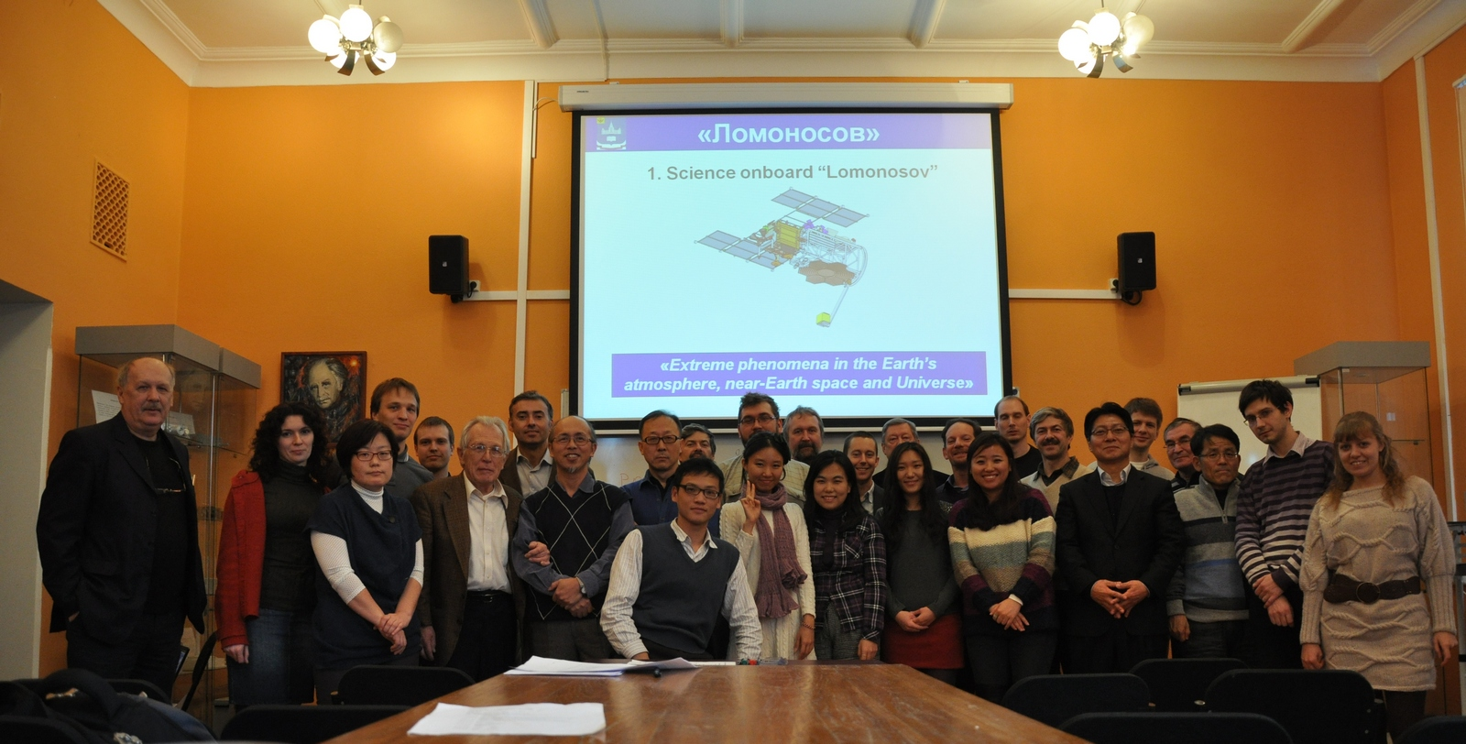
\includegraphics[width=0.7\linewidth]{images/collab}
	\caption{Коллаборация космического эксперимента Ломоносов}
	\label{fig:collab}
\end{figure}
